\documentclass[]{article}
\usepackage{graphicx}
\usepackage{float}
\usepackage[a4paper, total={6in, 8in}]{geometry}
\usepackage{geometry}
 \geometry{
 a4paper,
 total={170mm,257mm},
 left=20mm,
 top=20mm,
 }
\usepackage[shortlabels]{enumitem}


\begin{document}
\begin{titlepage}
    \begin{center}
        \vspace*{5cm}
            
        \Huge
        \textbf{CAB320 ASSIGNMENT 2}
            
        \vspace{0.5cm}
        \Huge
        \textbf{Transfer Learning}
            
        \vspace{1.5cm}
        
        \LARGE
        \textbf{Mitchell Egan}  n10210776
        
        \textbf{Jaydon Gunzburg}  n10396489  
        
        \textbf{Rodo Nguyen}  n10603280
        
    \end{center}
\end{titlepage}

\newpage

\section{Introduction}
The work conducted and analysed throughout this report seeks to adapt a Convolutional Neural Network (CNN) to identify 5 species of flower: Daisy, Dandelion, Rose, Sunflower and Tulip. The MobileNetV2 CNN, an architecture that seeks to perform on mobile devices, will be used as an initial, base network. The final layer of this network will be removed and replaced with an appropriate reductive neuron set to produce 5 classifiers for the 5 flower species (known as transfer learning). This network is then trained with Stochastic Gradient Descent (SGD) to optimise the objective function. The hyperparameters, learning rates and momentums, are varied to explore the effect they have on training processes and test accuracy.

\section{Data Preparation}
\subsection{Retrieval of the Provided Dataset}
The dataset of the five flower species was downloaded and briefly analysed. It was noted that some images under a particular classifier did not appear to completely conform to the description of that classifier, for example images of the word “roses” on a building or a billboard. Following the analysis, the dataset was loaded into the workspace. Each image was resized (whilst preserving its aspect ratio) to a desired size of 224 by 224 pixels (default MobileNetV2 input image resolution). The images were not converted to grey scale as colour was useful in recognising flowers. 8-bit pixel values of 3 RGB channels of each image were also normalised to be floating point values within the range of zero to one by dividing by 255 to reduce the complexity while training the neural network.

\subsection{Create Train, Validation \& Test Sets}
The dataset was distributed as a random 70/30 split between the training set and the combined validation and test sets. This choice is to ensure the model has the majority of data to train on. The validation and test sets were subsequently distributed randomly as a 50/50 from the remaining 30\% data. Figure \ref{fig:DataDistribution} presents the empirical allocation of these sets, confirming the desired distributions and demonstrating that the classifiers are also approximately equally divided within each set.

\begin{figure}[H]
  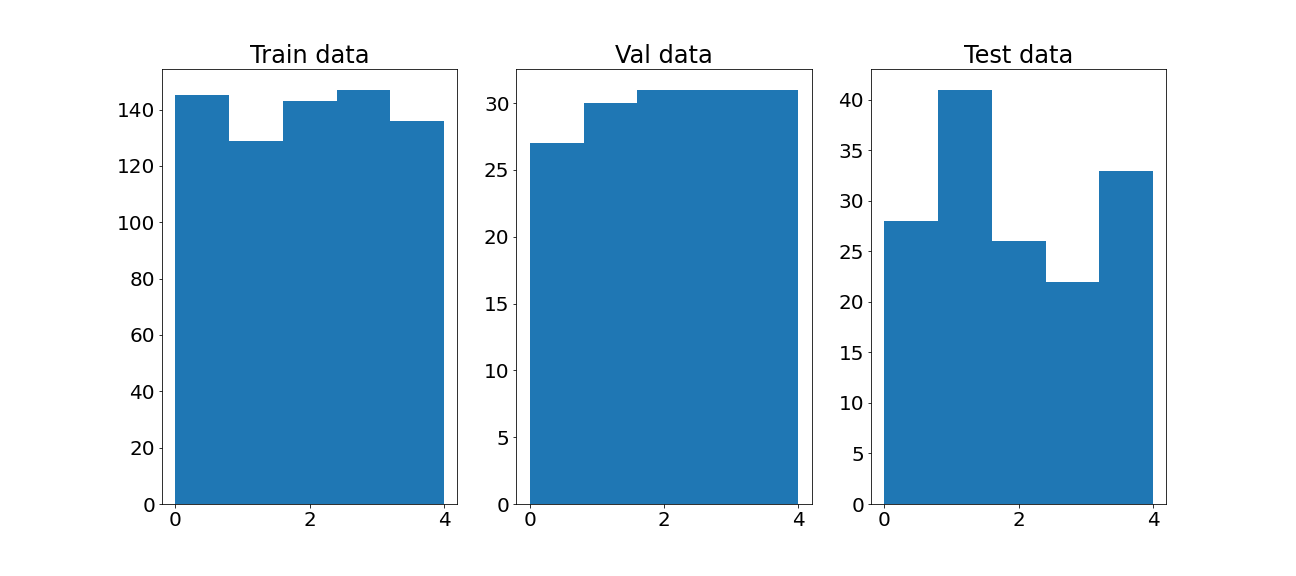
\includegraphics[scale=.25]{DataDistribution.png}
  \centering
  \caption{Data distribution between 5 classes in the train, validation and test sets}
  \label{fig:DataDistribution}
\end{figure}

\section{Model Preparation}
\subsection{Downloading and Layer Freezing}
The pretrained MobileNetV2 model was downloaded and initialised. It was configured to discard the top ImageNet fully-connected classifier layer, given that the classifier was to be retrained. Additionally, the pre-trained ImageNet weights were selected for use, as the ImageNet data would be relevant to the problem. Following initialisation, all layers of the model were frozen in order to retain their information until further actions (see Section \ref{training_process}). 

\subsection{Adding Layers}
Firstly, the MobileNetV2's last layer is connected to a Flatten layer to transform multi-dimensional input to one-dimensional output, which is a necessary transition from the convolution layer to the fully-connected layer ("Flatten", n.d.). There are five output classes, so the last layer was chosen to be a Dense layer with five outputs. However, several experiments were performed using different layer combinations after the Flatten layer:

\begin{itemize}
    \item E1: 2 Dense layers - fully-connect the previous one-dimensional layer to 64 outputs and then to the final 5 outputs.
    \item E2: 3 Dense - similar to 2 Dense layers, from 1024 to 64 to 5 outputs.
    \item E3: A single Dense layer with 5 outputs.   
\end{itemize}

Note that the last Dense layer uses the \textit{Soft Max} activation function to return the prediction probability for each class (which sum to one). The remaining Dense layers use the \textit{Rectified Linear Unit Activation Function} (ReLU) to deactivate neurons if their values are less than zero.

\begin{table}[H]
    \centering
    \begin{tabular}{ | c | c | }
     \hline
     Experiment model & Test Accuracy  \\ 
      \hline
        E1 & .913 \\  
      \hline
        E2 & .887 \\  
      \hline
        E3 & .867 \\  
      \hline
    \end{tabular}
    \caption{Experiment results of using different layer combinations.}
    \label{tab:LayerExperiments}
\end{table}

As can be seen from the experiment results in Table \ref{tab:LayerExperiments}, the model equipped with two Dense layers (E1) produced the highest accuracy in the test data (see also its last layers in Figure \ref{fig:Addedlayersshapes} below). As expected, the extra intermediate Dense layer adds more capacity to aggregate features and builds relationships between the convolutional layers and the final outputs. However, adding more Dense layers would hinder the learning ability, rather than assist the model.


\begin{figure}[H]
  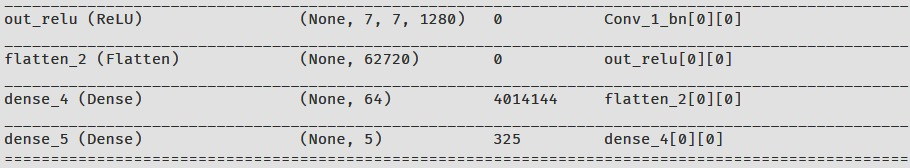
\includegraphics[scale=.45]{AddedLayersShapes.png}
  \centering
  \caption{The last layers added in E1.}
  \label{fig:Addedlayersshapes}
\end{figure}

An experiment was also performed by adding a BatchNorm and/or Dropout layer. In short, the BatchNorm layer takes the outputs from the previous hidden layer and normalises them, before passing them on as the input of the next hidden layer. This facilitates gradient descent (Teo, 2021). The Dropout layer randomly sets a portion of input units to zero for each step, which helps prevent overfitting ("Dropout layer", n.d.). However, the prediction accuracy drops compared to model E1 discussed above. It was speculated that the layers already added in the early convolutional blocks of MobileNetV2 are most helpful in maximising learning ability. Adding extra layers within the last fully-connected layers, responsible for classifying, only inhibits the prediction accuracy.

\subsection{Other Parameters}  \label{other_parameter}

\begin{enumerate}[(a)]
    \item SGD optimiser's parameters. \newline
    The default parameters of the SGD optimiser given are: learning rate = 0.01, momentum = 0.0, nesterov = False. Some of these were changed for each purpose as discussed in the Sections \ref{LRsection} and \ref{momentum_section}.  

    \item Loss function. \\
    A loss function is an indispensable parameter as the model uses it to self-evaluate how accurate it predicts. With each flower image to be classified into exactly one class, and each label is a single integer, Sparse Categorical Cross-entropy is utilised.


    \item Epoch number and batch size.  \\
    Each epoch uses a batch size of fifty and the maximum number of epochs is capped at 300. The batch size in this problem should be no less than five, else the model will not be exposed to a diverse batch at each step. The batch size should also not be too large, otherwise, there will be fewer steps per epoch that the model uses to update its weights. For example, a training set of 700 datapoints and a batch size of 100 allows the model to update 7 times per epoch. Hence, a batch size of 50 satisfies these two conditions. In fact, our experiments have shown that the model learns less effectively when training with a batch size of 25 (less than 50) or 100 (more than 50), meaning fifty is a reasonable batch size to train with. The experiment results are presented in Table \ref{tab:BatchSizeExperiments}, note that it was conducted with images resized to sixty-four by sixty-four pixels to compare the performance with different batch sizes as a main purpose while benefiting from training time reduction:
    
    \begin{table}[H]
    \centering
    \begin{tabular}{ | c | c | }
        \hline
        Batch size & Test Accuracy  \\ 
      \hline
        25 & .535 \\  
      \hline
        50 & .67 \\  
      \hline
        100 & .64 \\  
      \hline
    \end{tabular}
    \caption{Experiment results from using different batch sizes.}
    \label{tab:BatchSizeExperiments}
    \end{table}
    
    
    \item Callback functions.\\
    In order to save time and computational resources, 'Early Stopping' is added as one of the callbacks to stop the training after 20 epochs if there is no validation loss improvement. Another callback function is 'Model Checkpoint' which saves the models with both the lowest validation loss and highest validation accuracy. 
    
\end{enumerate}

\section{Training Process} \label{training_process}
There are two phases of the training process: train with the MobileNetV2 layers \textbf{frozen} and train with the MobileNetV2 layers \textbf{unfrozen}.

In \textbf{Phase 1}, all the layers from the MobileNetV2 are frozen and the newly added layers remain trainable. After the training finishes or is stopped by the Early Stopping function, weights from the model with the lowest validation loss are loaded. This is to avoid using the last version at the end of training which is subject to over-fitting.  

After that, in \textbf{Phase 2}, the model continues to train with all layers unfrozen in order to further adjust its weights in the early layers to adapt to this problem. Similarly to phase one, weights from the model with the lowest validation loss and the highest validation accuracy are loaded up for testing. 

The benefit of this process can be seen at the end of Section \ref{LRsection}

\section{Learning Rate Experimentation and Results} \label{LRsection}
First, the learning rate was set to 0.01 (default), followed by 3 different orders of magnitudes, 0.1, 0.001 and 0.0001. The aim was to show how the model trains and performs at different learning rates. From here, the most optimal learning rate could be chosen.

\subsection{Learning rate = 0.1} \label{LR01section}

Using a relatively high learning rate of 0.1, as seen on the left of Figure \ref{LR1}, the model started with a huge loss and then barely made any progress. The accuracy didn't improve throughout training and varies sporadically. This is most likely an example of a model 'orbiting' a local minimum. At first, the model made huge progress towards the goal because of such a large learning rate, but then, could not slowly decline into the local minimum as intended so it just kept oscillating around the point it was trying to reach. This also explains the accuracy fluctuating greatly and not improving. Moving to Phase 2, as all layers were set to trainable, more weights from the early layers of the model got over-adjusted as well and consequently worsened the performance as can be seen from its validation accuracy line in the right history plot of Figure \ref{LR1}. 

\begin{figure}[H]
  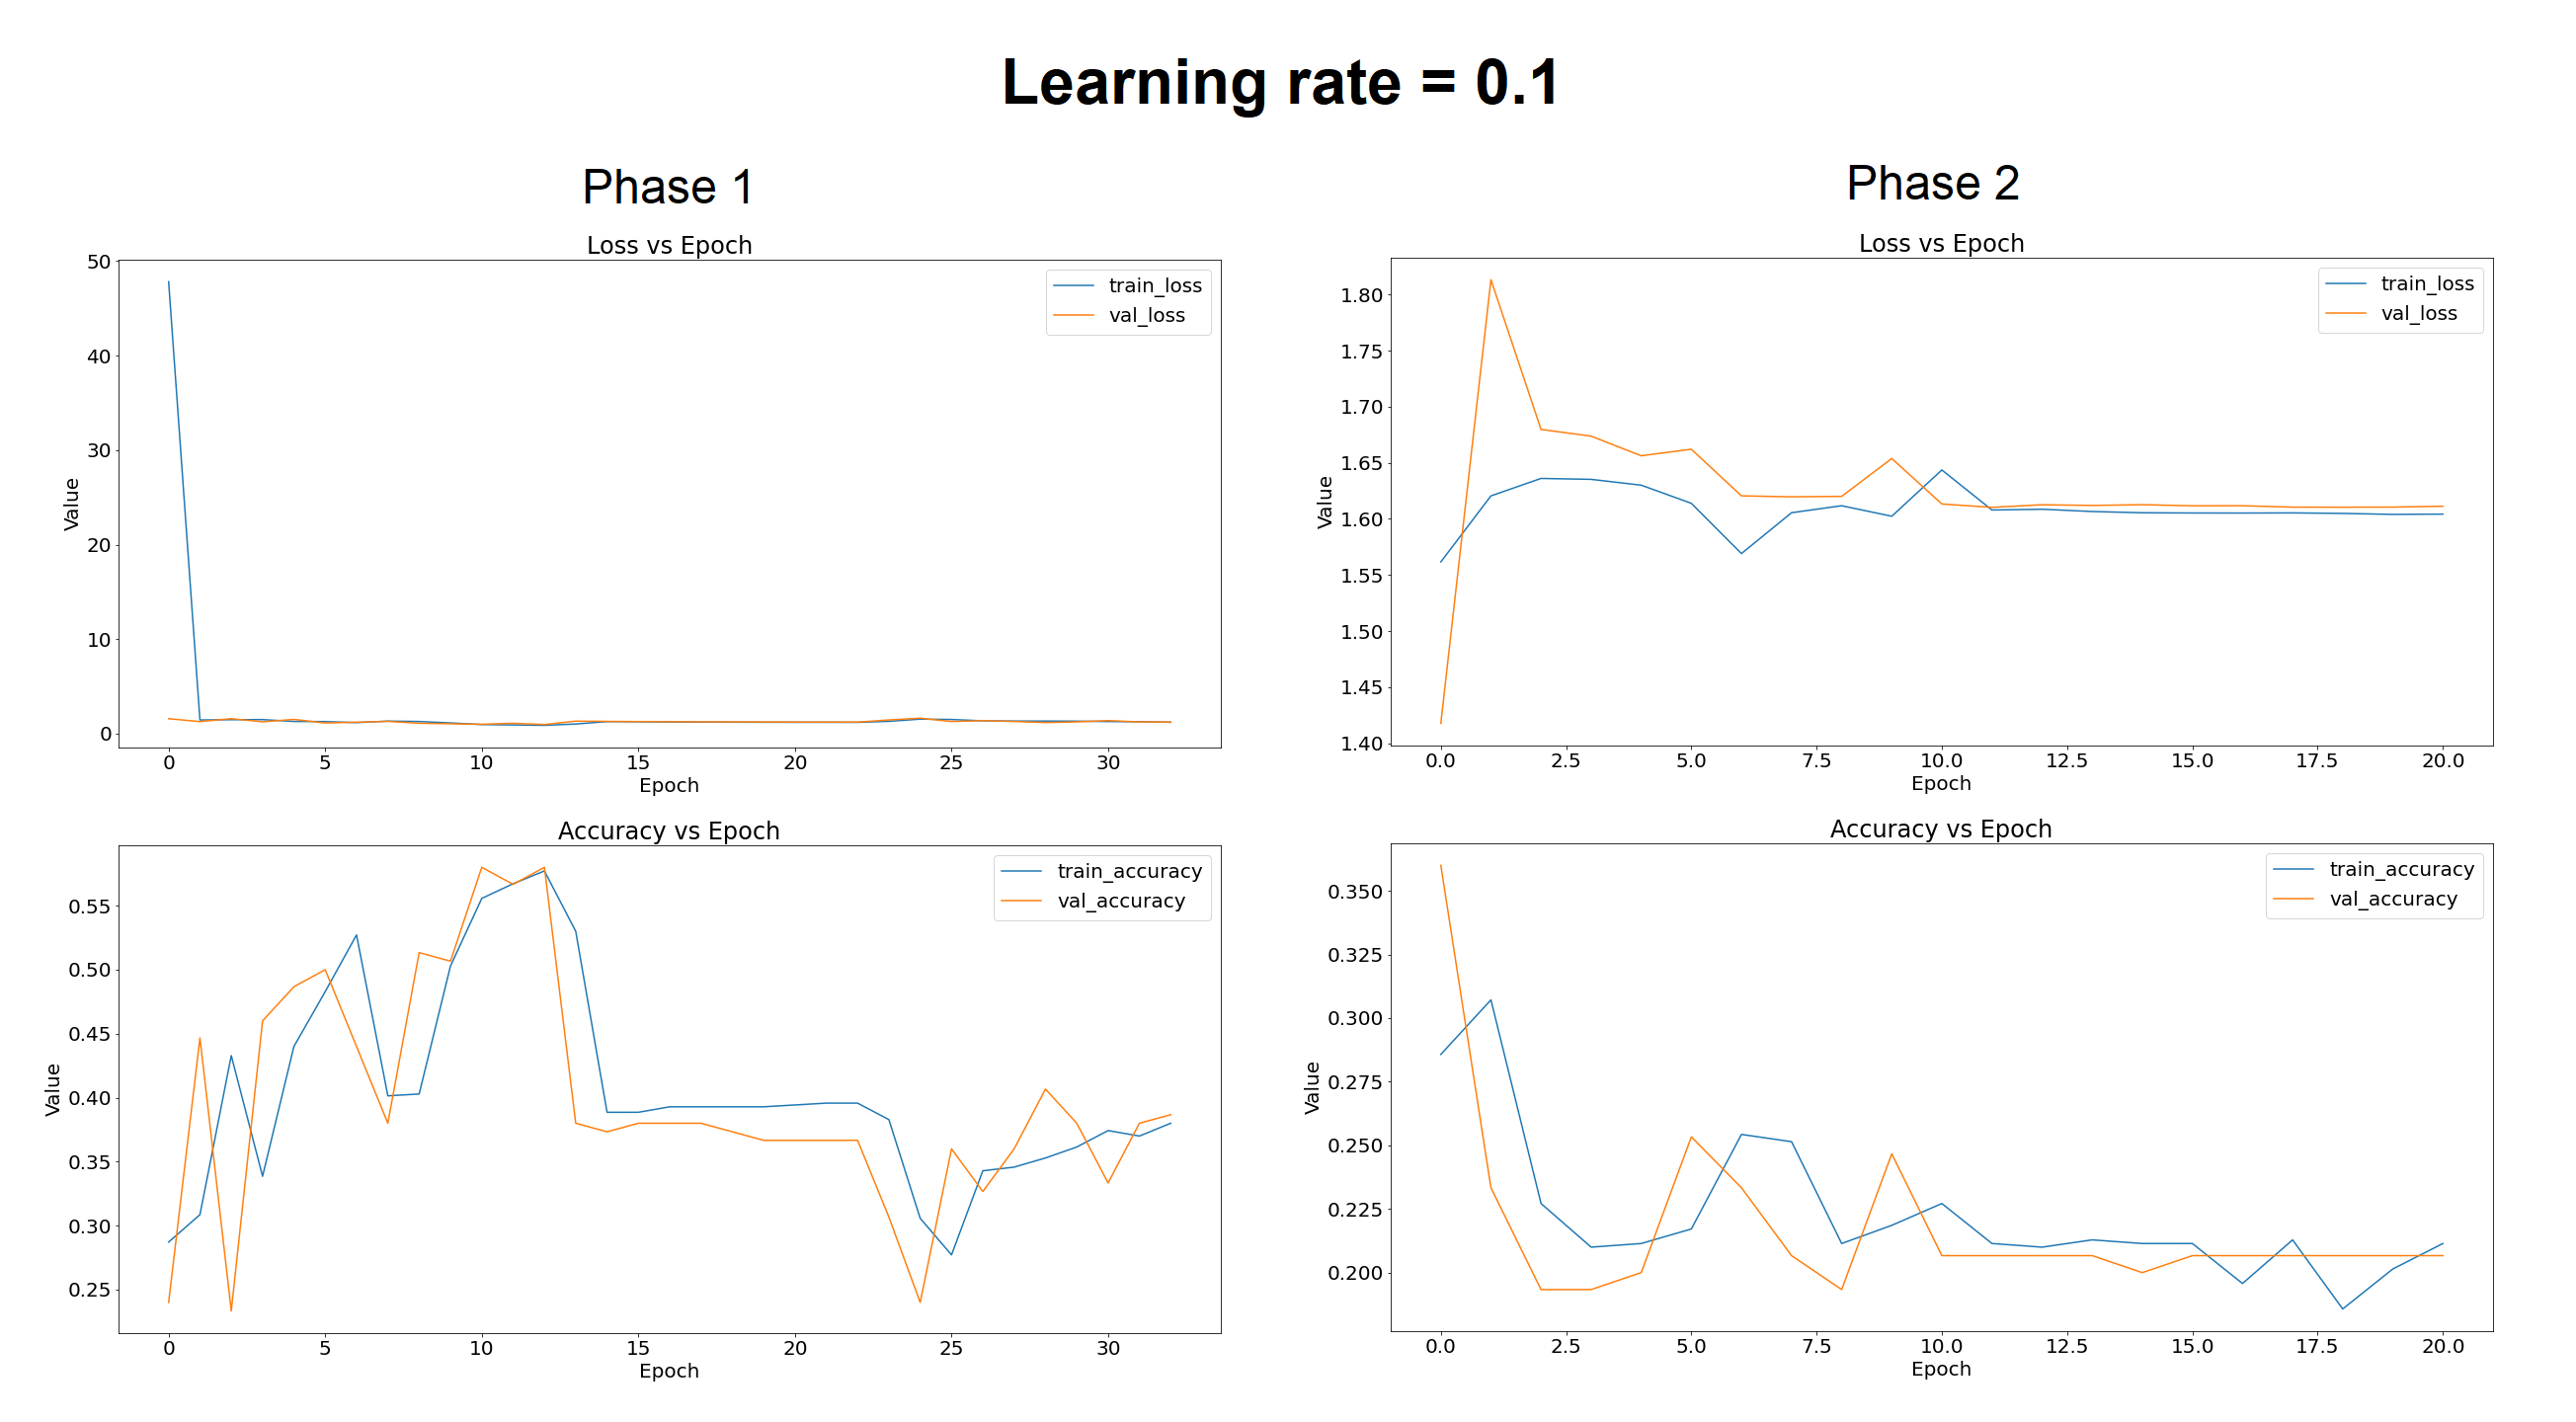
\includegraphics[scale=.16]{1_2P.png}
  \centering
  \caption{Learning rate = 0.1: training histories of both phases}
  \label{LR1}
\end{figure}

\subsection{Learning rate = 0.01} \label{LR001section}

The model trained with a 0.01 learning rate overall showed good progress in both validation loss and accuracy throughout both training Phases (Figure \ref{LR001}). A small peak in validation loss at the beginning of Phase 2 is speculated to be a process where the model was trying to adjust its weights of the recent unfrozen layers, which were pre-trained on another dataset, to now train on the new dataset. Other than that, no sign of overfitting (i.e., increasing loss or decreasing accuracy) is found in the training histories, which indicates a very stable training process. 

\begin{figure}[H]
  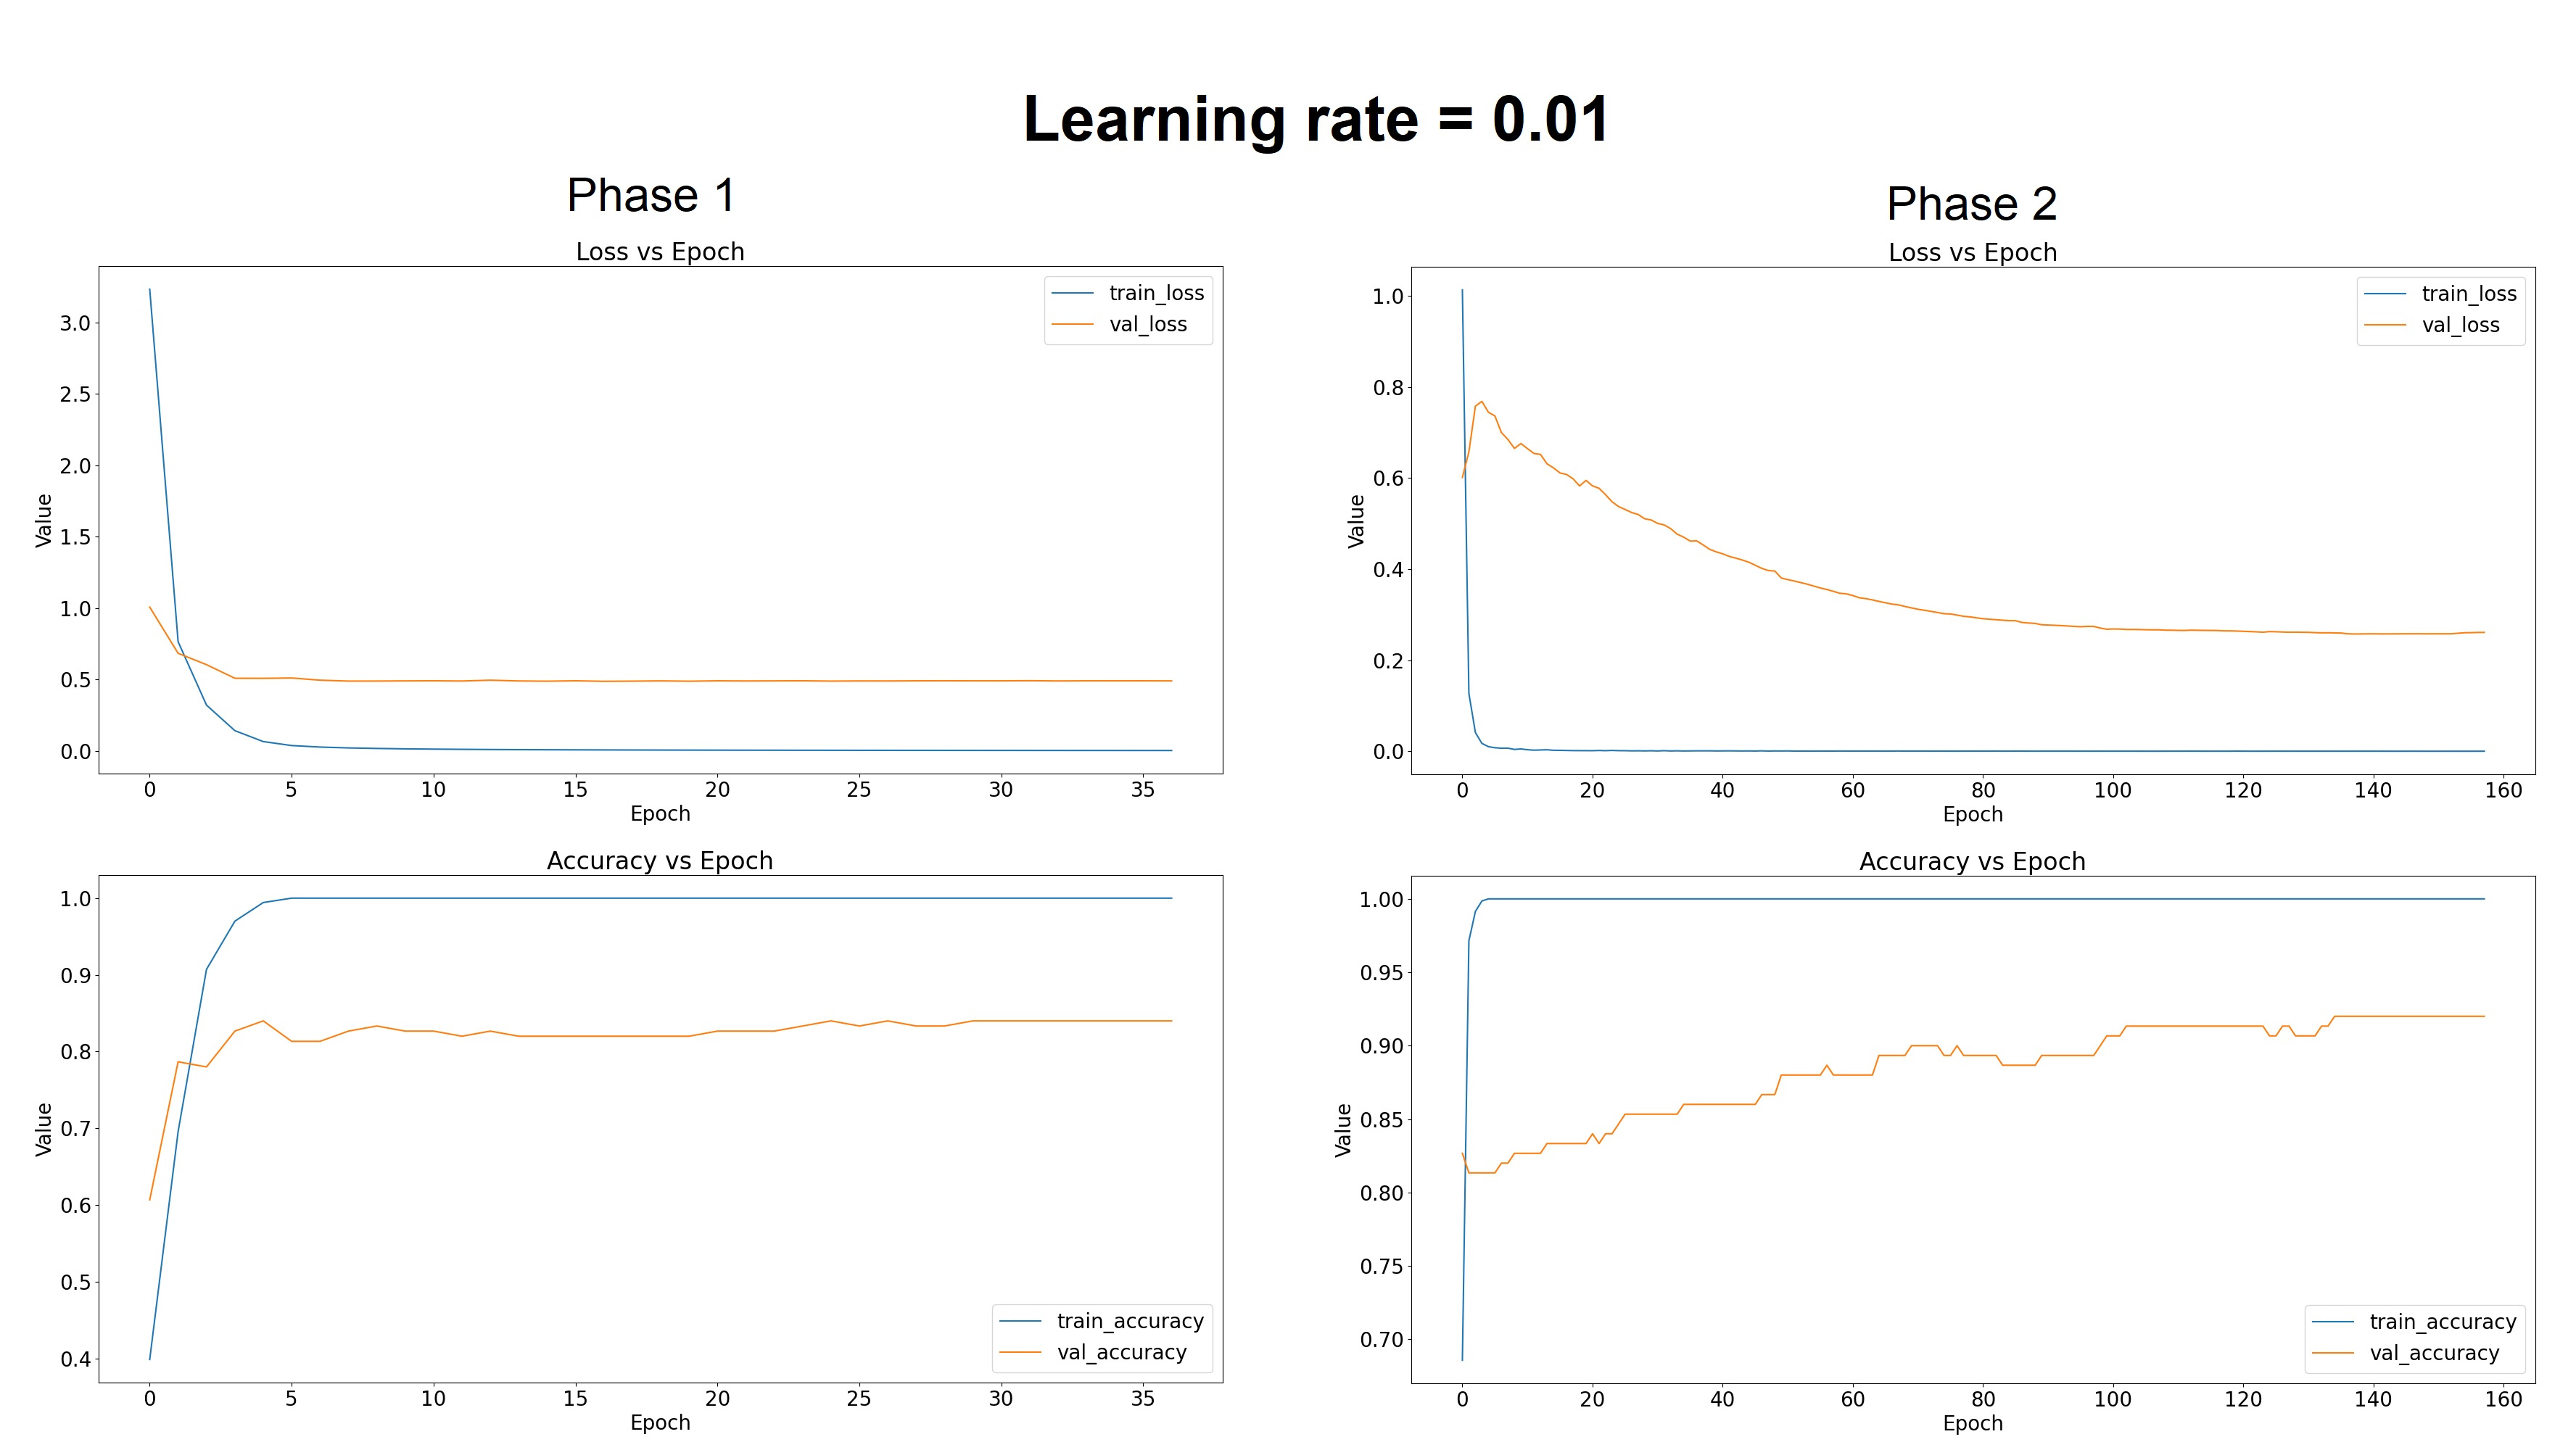
\includegraphics[scale=.11]{001_2P.png}
  \centering
  \caption{Learning rate = 0.01: training histories of both phases}
  \label{LR001}
\end{figure}

\subsection{Learning rate = 0.001 and 0.0001}

With lower learning rates, 0.001 and 0.0001, the models took a lot more epochs to train in phase 1. Both were still making progress in validation loss until epoch 300. The slower progress is illustrated by the long slowly-increasing lines of both validation loss and validation accuracy (see Figure \ref{fig:LR001andLR0001}). 

\begin{figure}[H]
  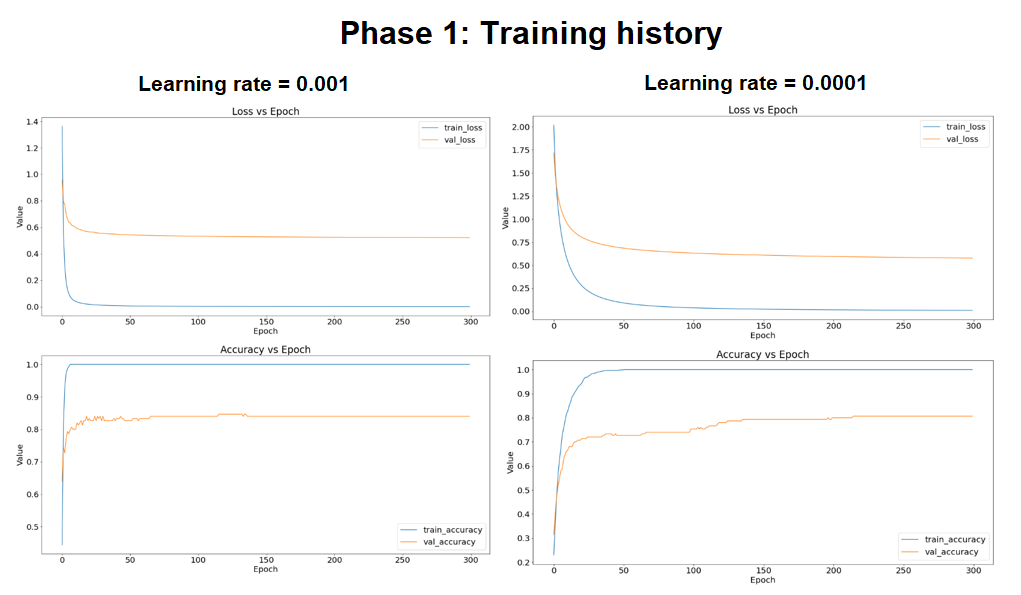
\includegraphics[scale=.37]{LR_0001_00001.png}
  \centering
  \caption{Model training in Phase 1 with a 0.001 and 0.0001 learning rate.}
  \label{fig:LR001andLR0001}
\end{figure}

Despite this can be seen as stable training, these 2 models got overfitted quickly in Phase 2. Their validation loss/validation accuracy reached optimal values around epoch 70 and decreased afterwards (see Figure \ref{fig:LR001andLR0001_P2}).

\begin{figure}[H]
  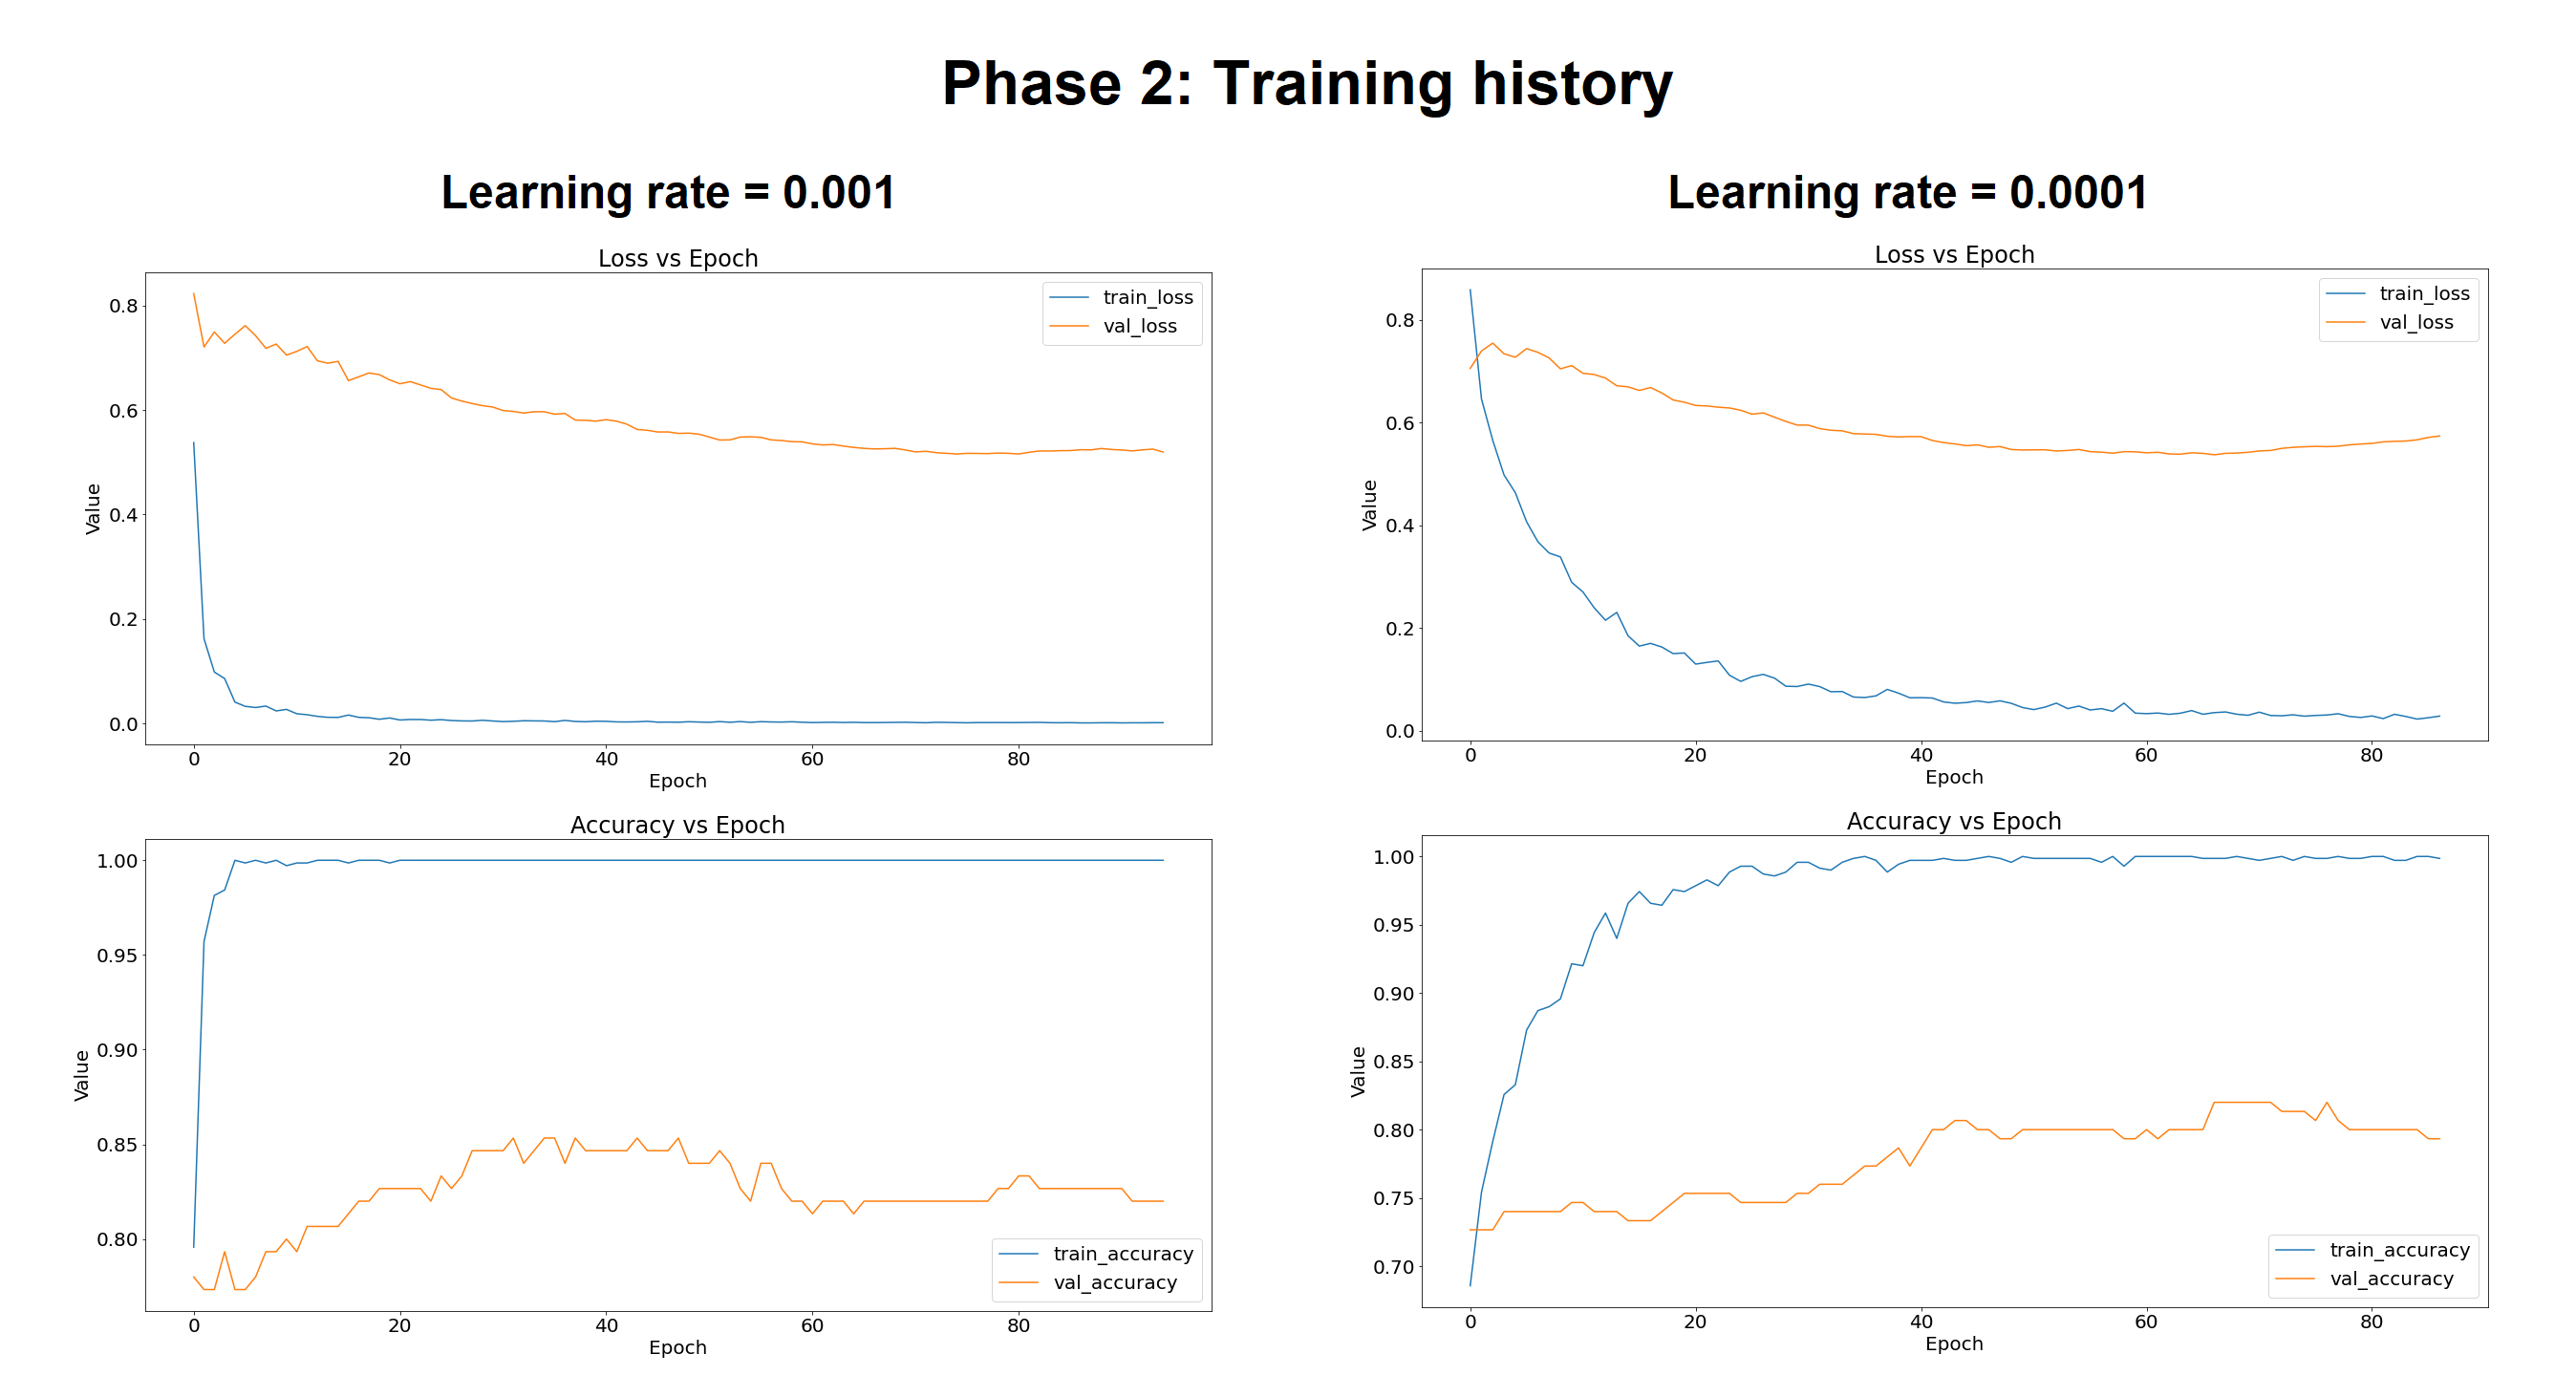
\includegraphics[scale=.15]{LR_0001_00001_unfreezeAllLayers.png}
  \centering
  \caption{Model training in Phase 2 with a 0.001 and 0.0001 learning rate.}
  \label{fig:LR001andLR0001_P2}
\end{figure}


\subsection{Summary \& Conclusion}

The test accuracy results from using 4 different learning rates are shown as below:
    \begin{table}[H]
    \centering
    \begin{tabular}{ | c | c | c |}
        \hline
        Learning rate & Phase 1: Test Accuracy & Phase 2: Test accuracy \\ 
      \hline
        0.1 & .53 & .31 \\ 
      \hline
        0.01 & .82 & .91 \\   
      \hline
        0.001 & .81 & .85 \\ 
      \hline
        0.0001 & .75 & .85 \\  
      \hline
    \end{tabular}
    \caption{Test accuracy results from using different learning rates}
    \label{tab:LRTestAccuracy}
    \end{table}
    
In summary, models using 0.001 and 0.001 learning rates showed a slow learning capability and were subject to overfitting with such long and slow training, not to mention our dataset is rather small for such complicated task and model architectures. Their highest test accuracy results were the same - 0.85. A large learning rate of 0.1 prevented the model from reaching local minimums, in other words, the model could not optimize its weights to learn the data properly. Unsurprisingly, its highest test accuracy was only 0.53 achieved in Phase 1.  

From the above performance discussion regarding experimenting with different learning rates, the model with a 0.01 learning rate displayed a stable training history and performed better than all the others in test data with a convincing accuracy of 0.91. Therefore, a learning rate of 0.01 was chosen for the proceeding section.  

Additionally, most results in Phase 2 are higher than those in Phase 1, which proved that unfreezing the early layers provided models more flexibility to continue to learn, adapt and perform better in the new problem. The models with all learning rates experiments, except for 0.1, have all benefited immensely from transfer learning with validation accuracy reaching 80\% in just 10 epochs.  


\section{Momentum Experimentation and Results} \label{momentum_section}

Momentum is an extension to the gradient descent optimization algorithm that allows the search to build inertia in a direction, overcome noise and coast across flat spots of the search space (Brownlee, 2021). In this section, 3 momentum values were chosen for experimenting: 

    \begin{itemize}
        \item M = 0.01: A small momentum value but not too insignificant to observe how it affects the performance. The results are expected to be similar to the one with 0 momentum
        \item M = 0.5: A medium value of momentum's valid range from 0 to 1  
        \item M = 1: The maximum value of momentum 
    \end{itemize}

\noindent All three models use 0.01 learning rate and the table below presents the results for each selected momentum values:
    \begin{table}[H]
    \centering
    \begin{tabular}{ | c | c | c | }
        \hline
        Momentum & Phase 1: Test Accuracy & Phase 2: Test accuracy \\ 
      \hline
        0.01 & .854 & .89 \\ 
      \hline
        0.5 & .826 & .878 \\   
      \hline
        1 & .61 & .43 \\ 
      \hline
    \end{tabular}
    \caption{Test accuracy results from using different momentums}
    \label{tab:MTestAccuracy}
    \end{table}

\subsection{Momentum = 0.01}

With 0.01 momentum, the model was able to learn and converge to the optimal performance faster in the training process as demonstrated by using fewer epochs (a total of 149 epochs compared to 194 epochs in the best model with a 0.01 learning rate found in Section \ref{LRsection}). It is also notable that in Phase 2, the model found it harder to climb back to .80 validation accuracy after falling from .85 in Phase 1 to .70 in epoch 1 Phase 2. Nevertheless, its test accuracy of 0.89 is a little lower than the best validation accuracy found at 0.91, which may indicate overfitting to the train data or that the model has not reached the local minimums. 


\begin{figure}[H]
  \includegraphics[scale=.15]{001.png}
  \centering
  \caption{Momentum = 0.01: training histories of both phases}
  \label{M_001}
\end{figure}

\subsection{Momentum = 0.5}

The model performed at an average level since the model achieved a test accuracy of .878 and the training also lasted for up to 175 epochs which is longer than most models' (see Figure \ref{M_05}). 

It still allowed the model to converge nicely in training history but reached the maximum validation accuracy at around epoch 110, which is much slower than the best model in Section \ref{LRsection} at epoch 70. So this momentum value can be considered to be relatively high. It allowed the model to learn well but the steps were not small enough for the model to adjust its weights to the optimal points. Thus, the validation accuracy plateaued at .88 and did not improve for the majority of the Phase 2 training.

\begin{figure}[H]
  \includegraphics[scale=.15]{05.png}
  \centering
  \caption{Momentum = 0.5: training histories of both phases}
  \label{M_05}
\end{figure}

\subsection{Momentum = 1}

With 1.0 momentum, the model behaviour was similar to what happened with the model using a 0.1 learning rate in Section \ref{LR01section} (see Figure \ref{M_10}). To be more specific, it could barely optimise its weights to the problem due to the extreme step updates that are boosted by the large momentum. This resulted in worsening performance during the training process which ended with a performance equaling random guess in Phase 2 (see Figure \ref{M_10}).


\begin{figure}[H]
  \includegraphics[scale=.15]{10.png}
  \centering
  \caption{Momentum = 1: training histories of both phases}
  \label{M_10}
\end{figure}

\subsection{Summary \& Conclusion}

In summary, adding the momentum value did not improve the test performance but also reduced it since their test accuracy results are all lower than the best one achieved in Section \ref{LRsection}. However, very small momentum values (such as 0.01 in the experiment) show good potential to assist the model to learn faster and reduce the training times but the performance change should be examined and considered carefully.

\section{Hyperparameters Recommendation}

From Section \ref{LRsection}, it was found that \textbf{0.01 learning rate} works best for this problem and provides a stable prediction result. In Section \ref{momentum_section}, \textbf{No momentum} value is found to be useful for increasing the model performance. 

However, different small momentum values can be further experimented with to improve the training time of the model while seeking to maintain or even improve the test accuracy. Similarly, experiments on nearby values of 0.01 (e.g, 0.011, 0.009, etc.) learning rate and \textit{nesterov} = True can be conducted for the same purpose. 


\newpage
\section{References}

\hspace{0.5cm}Brownlee, J. (2021, February 5). \textit{Gradient Descent With Momentum from Scratch}. Machinelearningmastery. https://machinelearningmastery.com/gradient-descent-with-momentum-from-scratch/

Doshi, K. (2021, May 19). \textit{Batch Norm Explained Visually — How it works, and why neural networks need it.} https://towardsdatascience.com/batch-norm-explained-visually-how-it-works-and-why-neural-networks-need-it-b18919692739

\textit{Dropout layer.} Keras. https://keras.io/api/layers/regularization\_layers/dropout/


\end{document}
